% !TeX root = ../Book3.tex
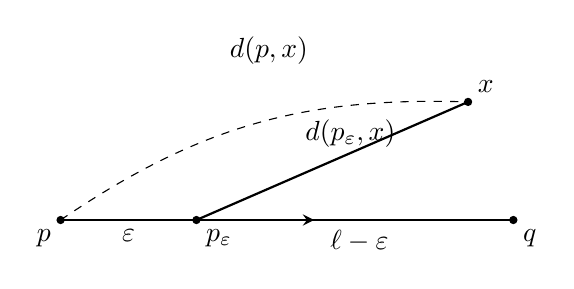
\begin{tikzpicture}[x=1.15cm,y=1cm,>=stealth]
	\coordinate (p) at (0,0);
	\coordinate (e) at (1.5,0);
	\coordinate (q) at (5,0);
	\coordinate (x) at (4.5,1.5);
	\draw[thick] (p)--(q);
	\draw[thick,->] (1.9,0)--(2.8,0);
	\draw[dashed] (p) to[bend left=18] (x);
	\draw[thick] (e)--(x);
	\node[above] at (2.3,1.85) {\(d(p,x)\)};
	\node[above,sloped] at (3.2,.8) {\(d(p_\varepsilon,x)\)};
	\node[below] at (.75,0) {\(\varepsilon\)};
	\node[below] at (3.3,0) {\(\ell-\varepsilon\)};
	\foreach \a in {p,e,q,x} {\fill (\a) circle (1.5pt);}
	\node[below left] at (p) {\(p\)};
	\node[below right] at (e) {\(p_\varepsilon\)};
	\node[below right] at (q) {\(q\)};
	\node[above right] at (x) {\(x\)};
\end{tikzpicture}
